\documentclass[11pt,a4paper]{article}

\usepackage[utf8]{inputenc}
\usepackage[indonesian]{babel}
\usepackage[a4paper,top=2cm,bottom=2cm,left=2cm,right=2cm]{geometry}
\usepackage{amsmath,amsfonts,amssymb}
\usepackage{graphicx}
\usepackage{booktabs}
\usepackage{array}
\usepackage{enumitem}
\usepackage{xcolor}
\usepackage{colortbl}
\usepackage{tcolorbox}
\usepackage{fancyhdr}
\usepackage{titlesec}
\usepackage[breaklinks=true,colorlinks=true,linkcolor=primaryblue,citecolor=primaryblue,urlcolor=primaryblue]{hyperref}

\definecolor{primaryblue}{RGB}{24, 43, 73}
\definecolor{secondaryblue}{RGB}{41, 128, 185}
\definecolor{boxbg}{RGB}{245, 248, 252}
\definecolor{goldaccent}{RGB}{211, 84, 0}
\definecolor{headerrow}{RGB}{24, 43, 73}

\pagestyle{fancy}
\fancyhf{}
\fancyhead[L]{\small\textbf{\color{primaryblue}Dokumen Deskripsi \& Manual Ciptaan HKI}}
\fancyhead[R]{\small\color{gray}TEE-412 / Teknik Elektro FT UNIB}
\fancyfoot[L]{\footnotesize\color{gray}Pencipta: Ir. Novalio Daratha, S.T., M.Sc., Ph.D.}
\fancyfoot[R]{\footnotesize Halaman \thepage}
\renewcommand{\headrulewidth}{0.5pt}
\renewcommand{\footrulewidth}{0.4pt}

\titleformat{\section}{\color{primaryblue}\normalfont\large\bfseries}{\thesection.}{0.5em}{}[\titlerule]
\titleformat{\subsection}{\color{secondaryblue}\normalfont\normalsize\bfseries}{\thesubsection}{0.5em}{}
\setlist{nosep}
\newcommand{\hdr}[1]{\cellcolor{headerrow}\color{white}\textbf{#1}}

\begin{document}

\begin{center}
    
\includegraphics[width=2.2cm]{../assets/logo_unib.png}\\[0.3cm]
    {\large \textbf{\color{primaryblue}UNIVERSITAS BENGKULU -- FAKULTAS TEKNIK}}\\[0.08cm]
    {\large \textbf{\color{secondaryblue}PROGRAM STUDI S1 TEKNIK ELEKTRO}}\\[0.25cm]
    {\LARGE \textbf{\color{primaryblue}DOKUMEN DESKRIPSI \& MANUAL CIPTAAN HKI}}\\[0.12cm]
    {\large \textbf{\color{goldaccent}PORTAL PEMBELAJARAN, VIRTUAL FORECASTING STUDIO, \& MODUL OBE}}\\
    {\large \textbf{\color{goldaccent}ANALISIS DERET WAKTU DAN PERAMALAN SISTEM TENAGA (TEE-412)}}\\[0.1cm]
    {\normalsize Lampiran Pengajuan Pencatatan Hak Cipta DJKI / LPPM Universitas Bengkulu}
\end{center}

\vspace{0.25cm}

\begin{tcolorbox}[colback=boxbg,colframe=primaryblue,arc=2mm,title=\textbf{Identitas Pencipta \& Informasi Ciptaan}]
\small
\setlength{\tabcolsep}{4pt}
\begin{tabular}{p{4.1cm}p{11.4cm}}
\textbf{Pencipta} & : Ir. Novalio Daratha, S.T., M.Sc., Ph.D. (NIP. 197811102003121002) \\
\textbf{Pemegang Hak Cipta} & : Universitas Bengkulu / LPPM Universitas Bengkulu \\
\textbf{Jenis Ciptaan 1} & : \textbf{Program Komputer} -- Portal Web Interaktif \& Virtual Forecasting Studio (\texttt{TEE-412}) \\
\textbf{Jenis Ciptaan 2} & : \textbf{Buku / Modul Ajar} -- Ekosistem Bahan Ajar, Praktikum, \& Bank Soal OBE C1--C6 \\
\textbf{Tanggal Publikasi Pertama} & : Agustus -- November 2026 (Bengkulu, Indonesia) \\
\textbf{URL Akses Publik} & : \url{https://www.ndaratha.my.id/deret-waktu} \\
\textbf{Repositori Kode Sumber} & : \url{https://github.com/novatha/deret-waktu-tee412} \\
\end{tabular}
\end{tcolorbox}

\section{Ringkasan Eksekutif \& Nilai Kebaruan Ciptaan}

Ciptaan ini merupakan ekosistem pembelajaran terbuka terintegrasi untuk mata kuliah \textbf{Analisis Deret Waktu dan Peramalan (\texttt{TEE-412}, 3 SKS)} pada Program Studi S1 Teknik Elektro, Fakultas Teknik Universitas Bengkulu. Kebaruan utama karya ini terletak pada penggabungan empat pilar dalam satu arsitektur terpadu:
\begin{enumerate}[label=\textbf{\arabic*.}, leftmargin=1.5em, itemsep=3pt]
    \item \textbf{Spesialisasi Domain Sistem Tenaga \& Transisi Energi:} Seluruh formulasi matematis, dataset, dan studi kasus dirancang khusus untuk sistem tenaga modern (beban harian PLN, intermitensi PLTS/PLTB, suhu transformator, SoC baterai BESS, harmonisa motor, dan deteksi pencurian listrik \textit{smart meter}).
    \item \textbf{Virtual Forecasting Studio Berbasis Browser (100\% Kausal):} Menyediakan laboratorium komputasi \textit{real-time} di sisi klien tanpa server backend, menjalankan 4 estimator kausal sejati (\textit{Discrete Kalman Filter}, \textit{Holt-Winters}, \textit{SARIMA}, dan \textit{Recurrent LSTM Emulator}) serta fitur \textbf{Upload CSV Mandiri} dan ekspor hasil eksperimen.
    \item \textbf{Praktikum \textit{Zero-Setup} Berbasis Cloud:} 12 berkas notebook interaktif (\texttt{.ipynb}) siap dijalankan 1-klik melalui Google Colab, disertai 3 dataset CSV kurasi terintegrasi otomatis (lokal/GitHub raw URL), protokol anti-\textit{data leakage}, dan validasi otomatis GitHub Actions CI.
    \item \textbf{Kepatuhan Penuh Kurikulum OBE (LAM Teknik / IABEE):} Menyelaraskan RPS 16 minggu (bobot tervalidasi 100\%), 13 modul slide Beamer, 13 \textit{Problem Sets} dan 13 \textit{Worksheets} berjenjang Taksonomi Bloom C1--C6, buku panduan praktikum 12 bab, 39 kuis \textit{self-check} interaktif, panduan \& template laporan proyek akhir IEEE 2-kolom, serta instrumen evaluasi OBE-CQI (PDCA).
\end{enumerate}

\section{Spesifikasi Teknis Ciptaan 1 -- Program Komputer}

\subsection{Arsitektur Perangkat Lunak}
\begin{itemize}[leftmargin=1.5em, itemsep=2pt]
    \item \textbf{Kerangka Kerja Web:} Astro 7 (Static Site Generation, 18 rute statis terkompilasi, ukuran total $\sim 11$ MB termasuk aset PDF dan notebook).
    \item \textbf{Komputasi Visual \& Matematis Lokal:} Chart.js 4 untuk plot interaktif multi-kanal, KaTeX (CSS + 19 berkas font \texttt{.woff2} terbundel lokal) untuk rendering persamaan LaTeX, serta ikon Lucide ter-\textit{tree-shake} lokal (bebas gangguan CDN skrip pihak ketiga).
    \item \textbf{Mesin Estimator Kausal (\texttt{ForecastingStudio.astro}):}
    \begin{enumerate}[label=(\alph*)]
        \item \textit{Discrete Kalman Filter (BLUE):} Rekursi prediksi--koreksi dengan kontrol interaktif matriks $Q$ dan $R$ serta proyeksi horizon musiman.
        \item \textit{Holt-Winters Triple Smoothing:} Pembaruan level ($\alpha$), tren ($\beta$), dan musiman ($\gamma$) berperiode $S \le 24$.
        \item \textit{Causal SARIMA(1,0,1)(0,1,0)[24]:} Diferensiasi musiman murni + estimasi autokorelasi AR(1) dan inovasi MA(1) hanya dari data sensor historis.
        \item \textit{Causal Recurrent LSTM / Reservoir Emulator:} Lapisan \textit{leaky tanh} rekuren 6-unit dengan pembacaan \textit{Ridge Regression} terlatih kausal di browser tanpa kebocoran target (\textit{zero truth leakage}).
    \end{enumerate}
    \item \textbf{Modul Unggah CSV Mandiri:} Mendukung unggahan berkas \texttt{.csv} (pemisah koma/titik-koma), deteksi otomatis kolom waktu dan numerik hingga 168 titik terakhir, perhitungan langsung RMSE, MAE, MAPE, $R^2$, serta ekspor hasil ke CSV.
\end{itemize}

\subsection{Panduan Singkat Penggunaan Aplikasi}
\begin{enumerate}[label=\textbf{\arabic*.}, leftmargin=1.5em, itemsep=2pt]
    \item Buka \url{https://www.ndaratha.my.id/deret-waktu} melalui peramban web modern (desktop/mobile).
    \item Akses menu \textbf{Silabus \& RPS} untuk mengunduh RPS OBE, Kisi-Kisi UTS/UAS, Panduan Proyek Akhir, dan Template LaTeX IEEE.
    \item Akses menu \textbf{13 Modul Perkuliahan} untuk mempelajari rumus, mengerjakan \textbf{Kuis Self-Check Interaktif}, menyalin cuplikan kode Python, dan mengunduh Slide Beamer, Soal C1--C6, serta Worksheet.
    \item Akses menu \textbf{Panduan Praktikum} untuk mengunduh Buku Praktikum PDF, mengunduh dataset CSV, atau membuka 12 notebook praktikum secara langsung lewat tombol \textbf{Buka di Colab}.
    \item Akses menu \textbf{Virtual Lab Studio} untuk menyimulasikan derau sensor, membandingkan 4 estimator, mengunggah dataset CSV mandiri, dan mengekspor hasil simulasi.
\end{enumerate}

\section{Spesifikasi Ciptaan 2 -- Modul Ajar \& Bank Soal OBE}

{\footnotesize
\setlength{\tabcolsep}{4pt}
\begin{tabular}{|p{3.8cm}|p{2.3cm}|p{9.2cm}|}
\hline
\hdr{Komponen Karya Tulis} & \hdr{Volume Sumber} & \hdr{Cakupan Substansi Akademik} \\ \hline
RPS OBE (Markdown \& LaTeX) & 16 Minggu & Pemetaan CPL 1--4, CPMK 1--5, Sub-CPMK 1--14, bobot penilaian, \& 8 tema PjBL \\ \hline
Slide Perkuliahan Beamer & 13 Modul (2.904 baris) & Minggu 1--7 (Dekomposisi s.d. Kalman Filter) \& Minggu 9--14 (FFT/Wavelet s.d. BESS MPC) \\ \hline
Problem Sets \& Worksheets & 26 Set (2.996 baris) & Soal terstruktur berjenjang Taksonomi Bloom C1 (10\%) s.d. C6 (20\%) tiap minggu \\ \hline
Buku Panduan Praktikum & 12 Bab (648 baris) & Implementasi Python (\texttt{statsmodels}, \texttt{PyWavelets}, \texttt{xgboost}, \texttt{PyTorch}, \texttt{scipy}) \\ \hline
Panduan Proyek Akhir IEEE & 1 Panduan + Template & Protokol anti-\textit{leakage}, deklarasi AI, rubrik 25\%, \& template \texttt{IEEEtran} 2-kolom \\ \hline
\end{tabular}
}

\section{Pernyataan Orisinalitas}

Dokumen ini disusun sebagai bahan pendukung pencatatan Hak Cipta di Direktorat Jenderal Kekayaan Intelektual (DJKI) melalui LPPM Universitas Bengkulu. Seluruh naskah bahan ajar, rancangan struktur soal C1--C6, 12 notebook praktikum, serta kode antarmuka dan mesin simulasi portal disusun secara orisinal untuk kepentingan pendidikan tinggi, penelitian, dan pengabdian masyarakat pada Program Studi S1 Teknik Elektro, Fakultas Teknik Universitas Bengkulu.

\vspace{0.5cm}
\noindent
\begin{tabular}{p{9.5cm}p{6cm}}
 & Bengkulu, November 2026 \\
 & Pencipta, \\[1.5cm]
 & \textbf{Ir. Novalio Daratha, S.T., M.Sc., Ph.D.} \\
 & NIP. 197811102003121002 \\
\end{tabular}

\newpage
\section*{Lampiran A: Tangkapan Layar Antarmuka Portal \& Virtual Lab Studio}
\addcontentsline{toc}{section}{Lampiran A: Tangkapan Layar Antarmuka Portal \& Virtual Lab Studio}

Berikut adalah dokumentasi visual aktual antarmuka \textbf{Ciptaan 1 (Program Komputer)} yang dirender langsung dari build produksi Astro 7 (\url{https://www.ndaratha.my.id/deret-waktu}):

\begin{figure}[h!]
    \centering
    \fbox{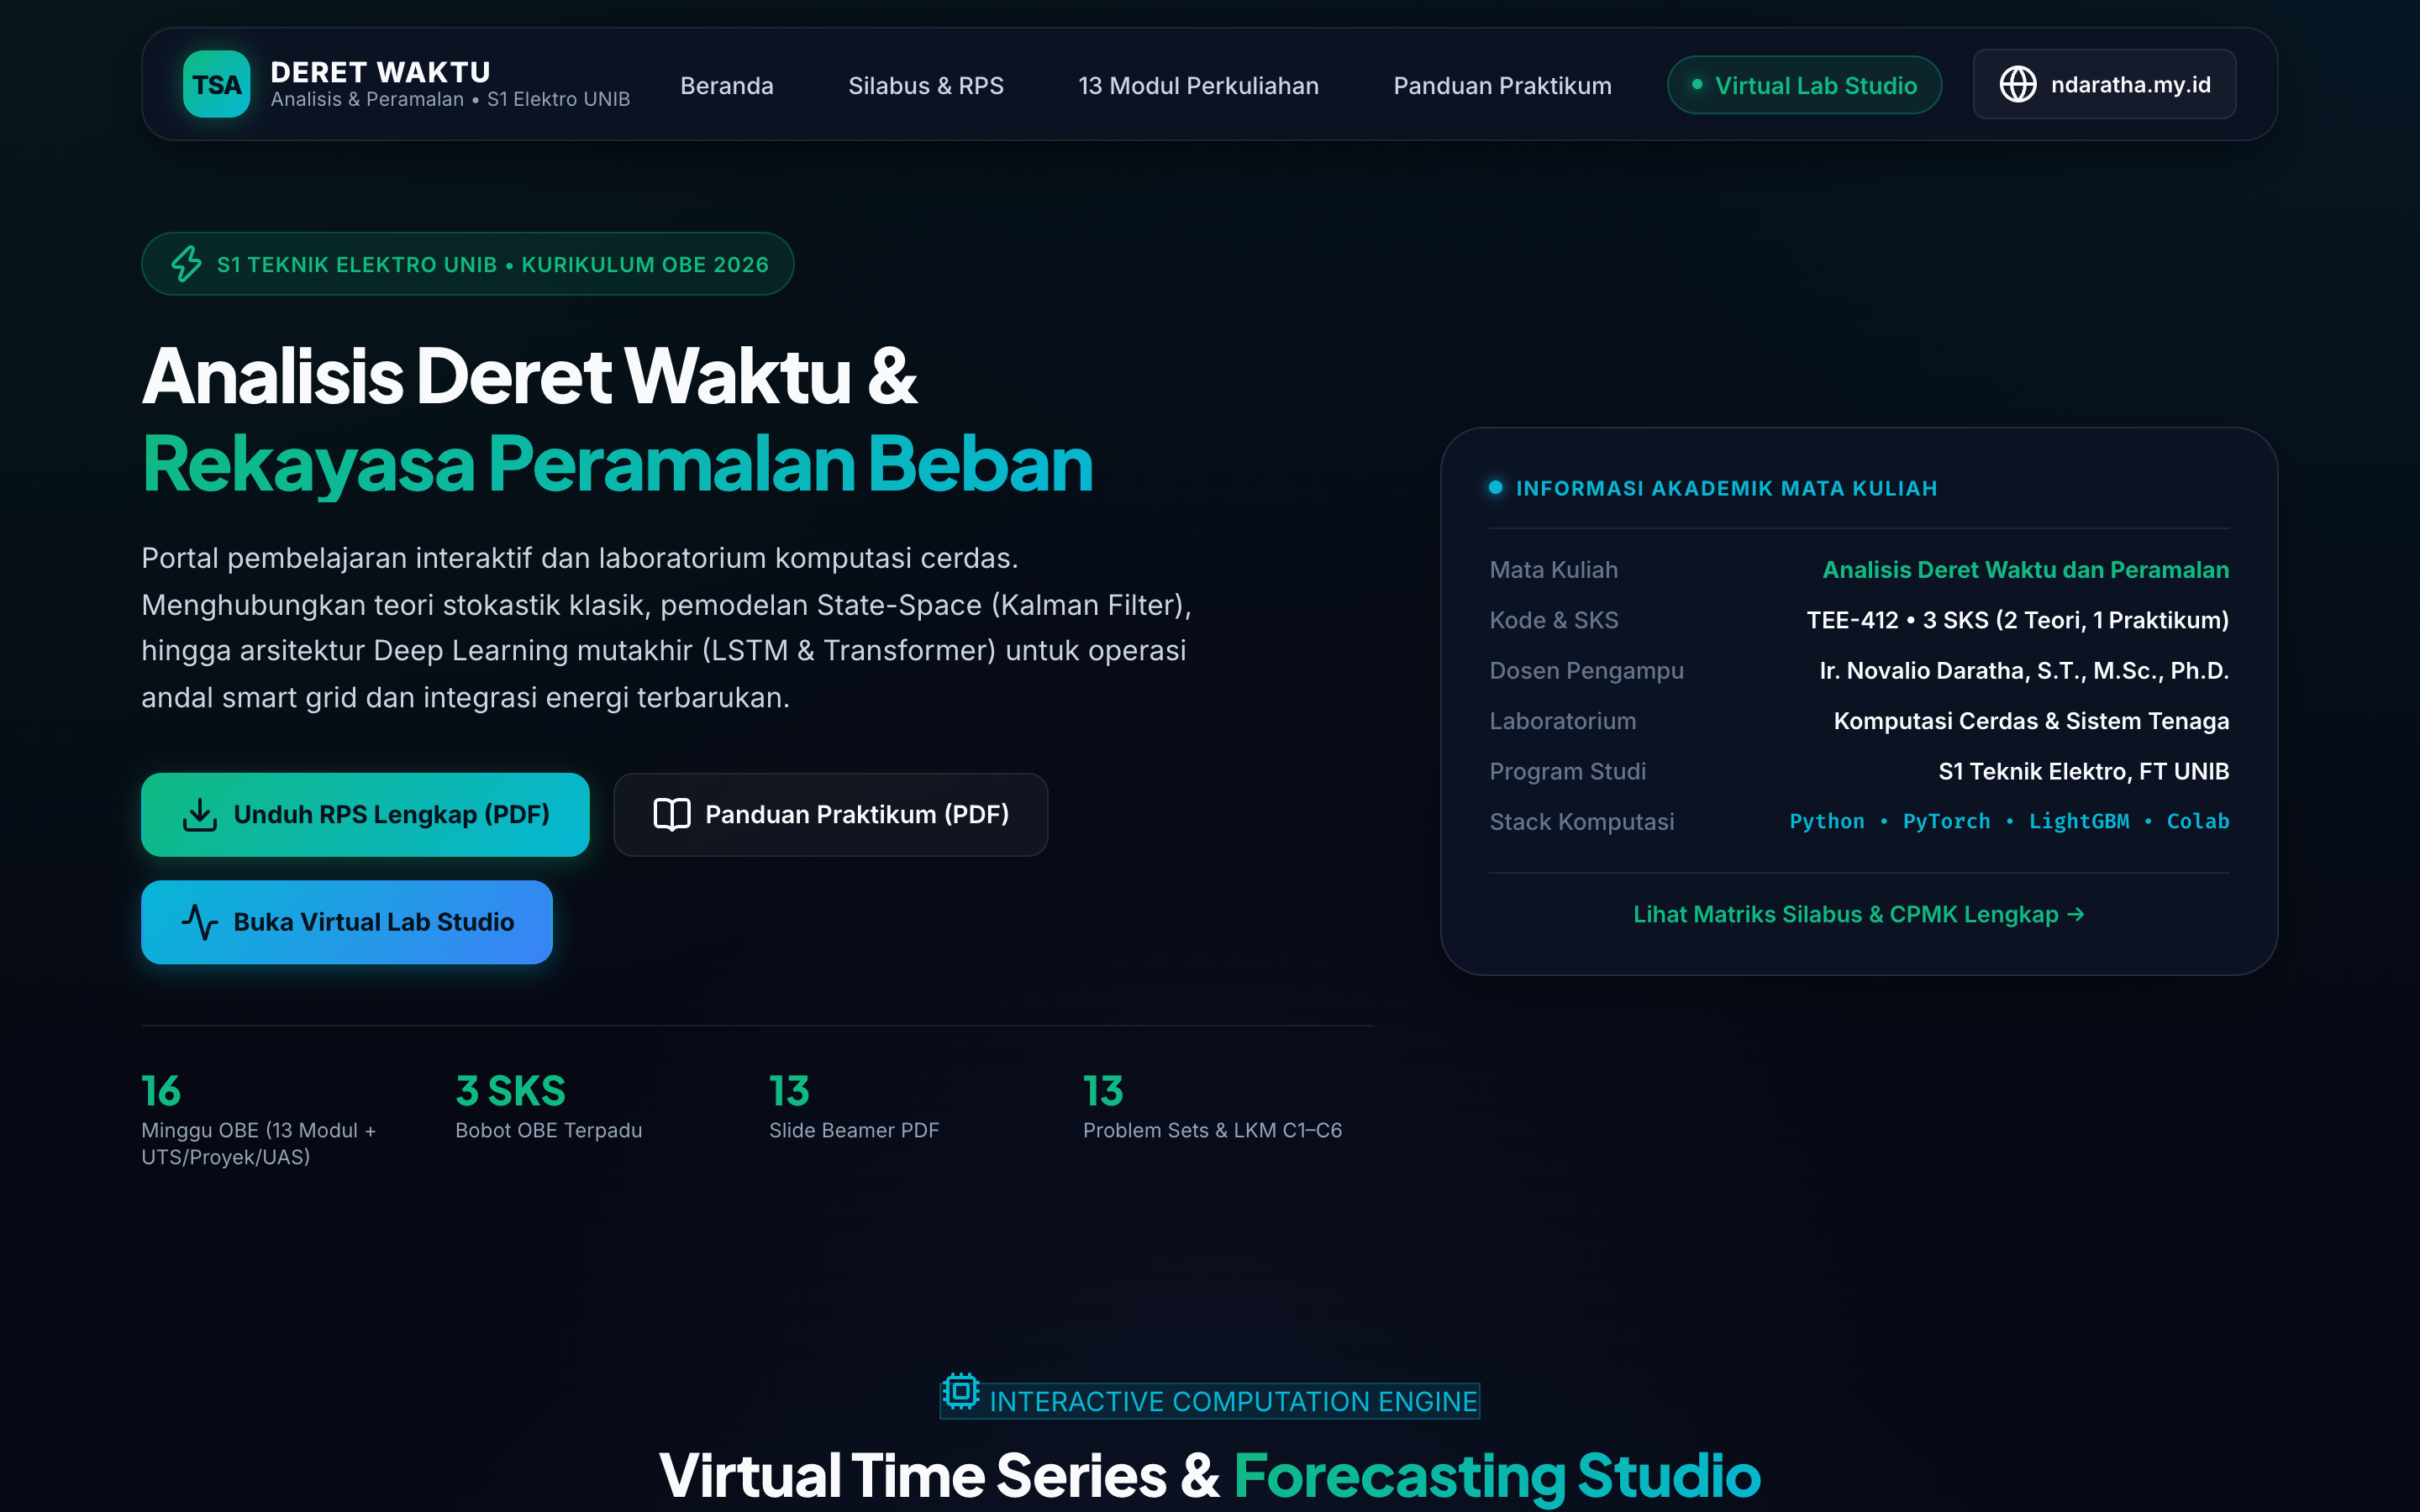
\includegraphics[width=0.92\textwidth]{screenshots/01_beranda_portal.png}}
    \caption{Halaman Beranda Portal Pembelajaran Terbuka Analisis Deret Waktu \& Peramalan (TEE-412).}
\end{figure}

\begin{figure}[h!]
    \centering
    \fbox{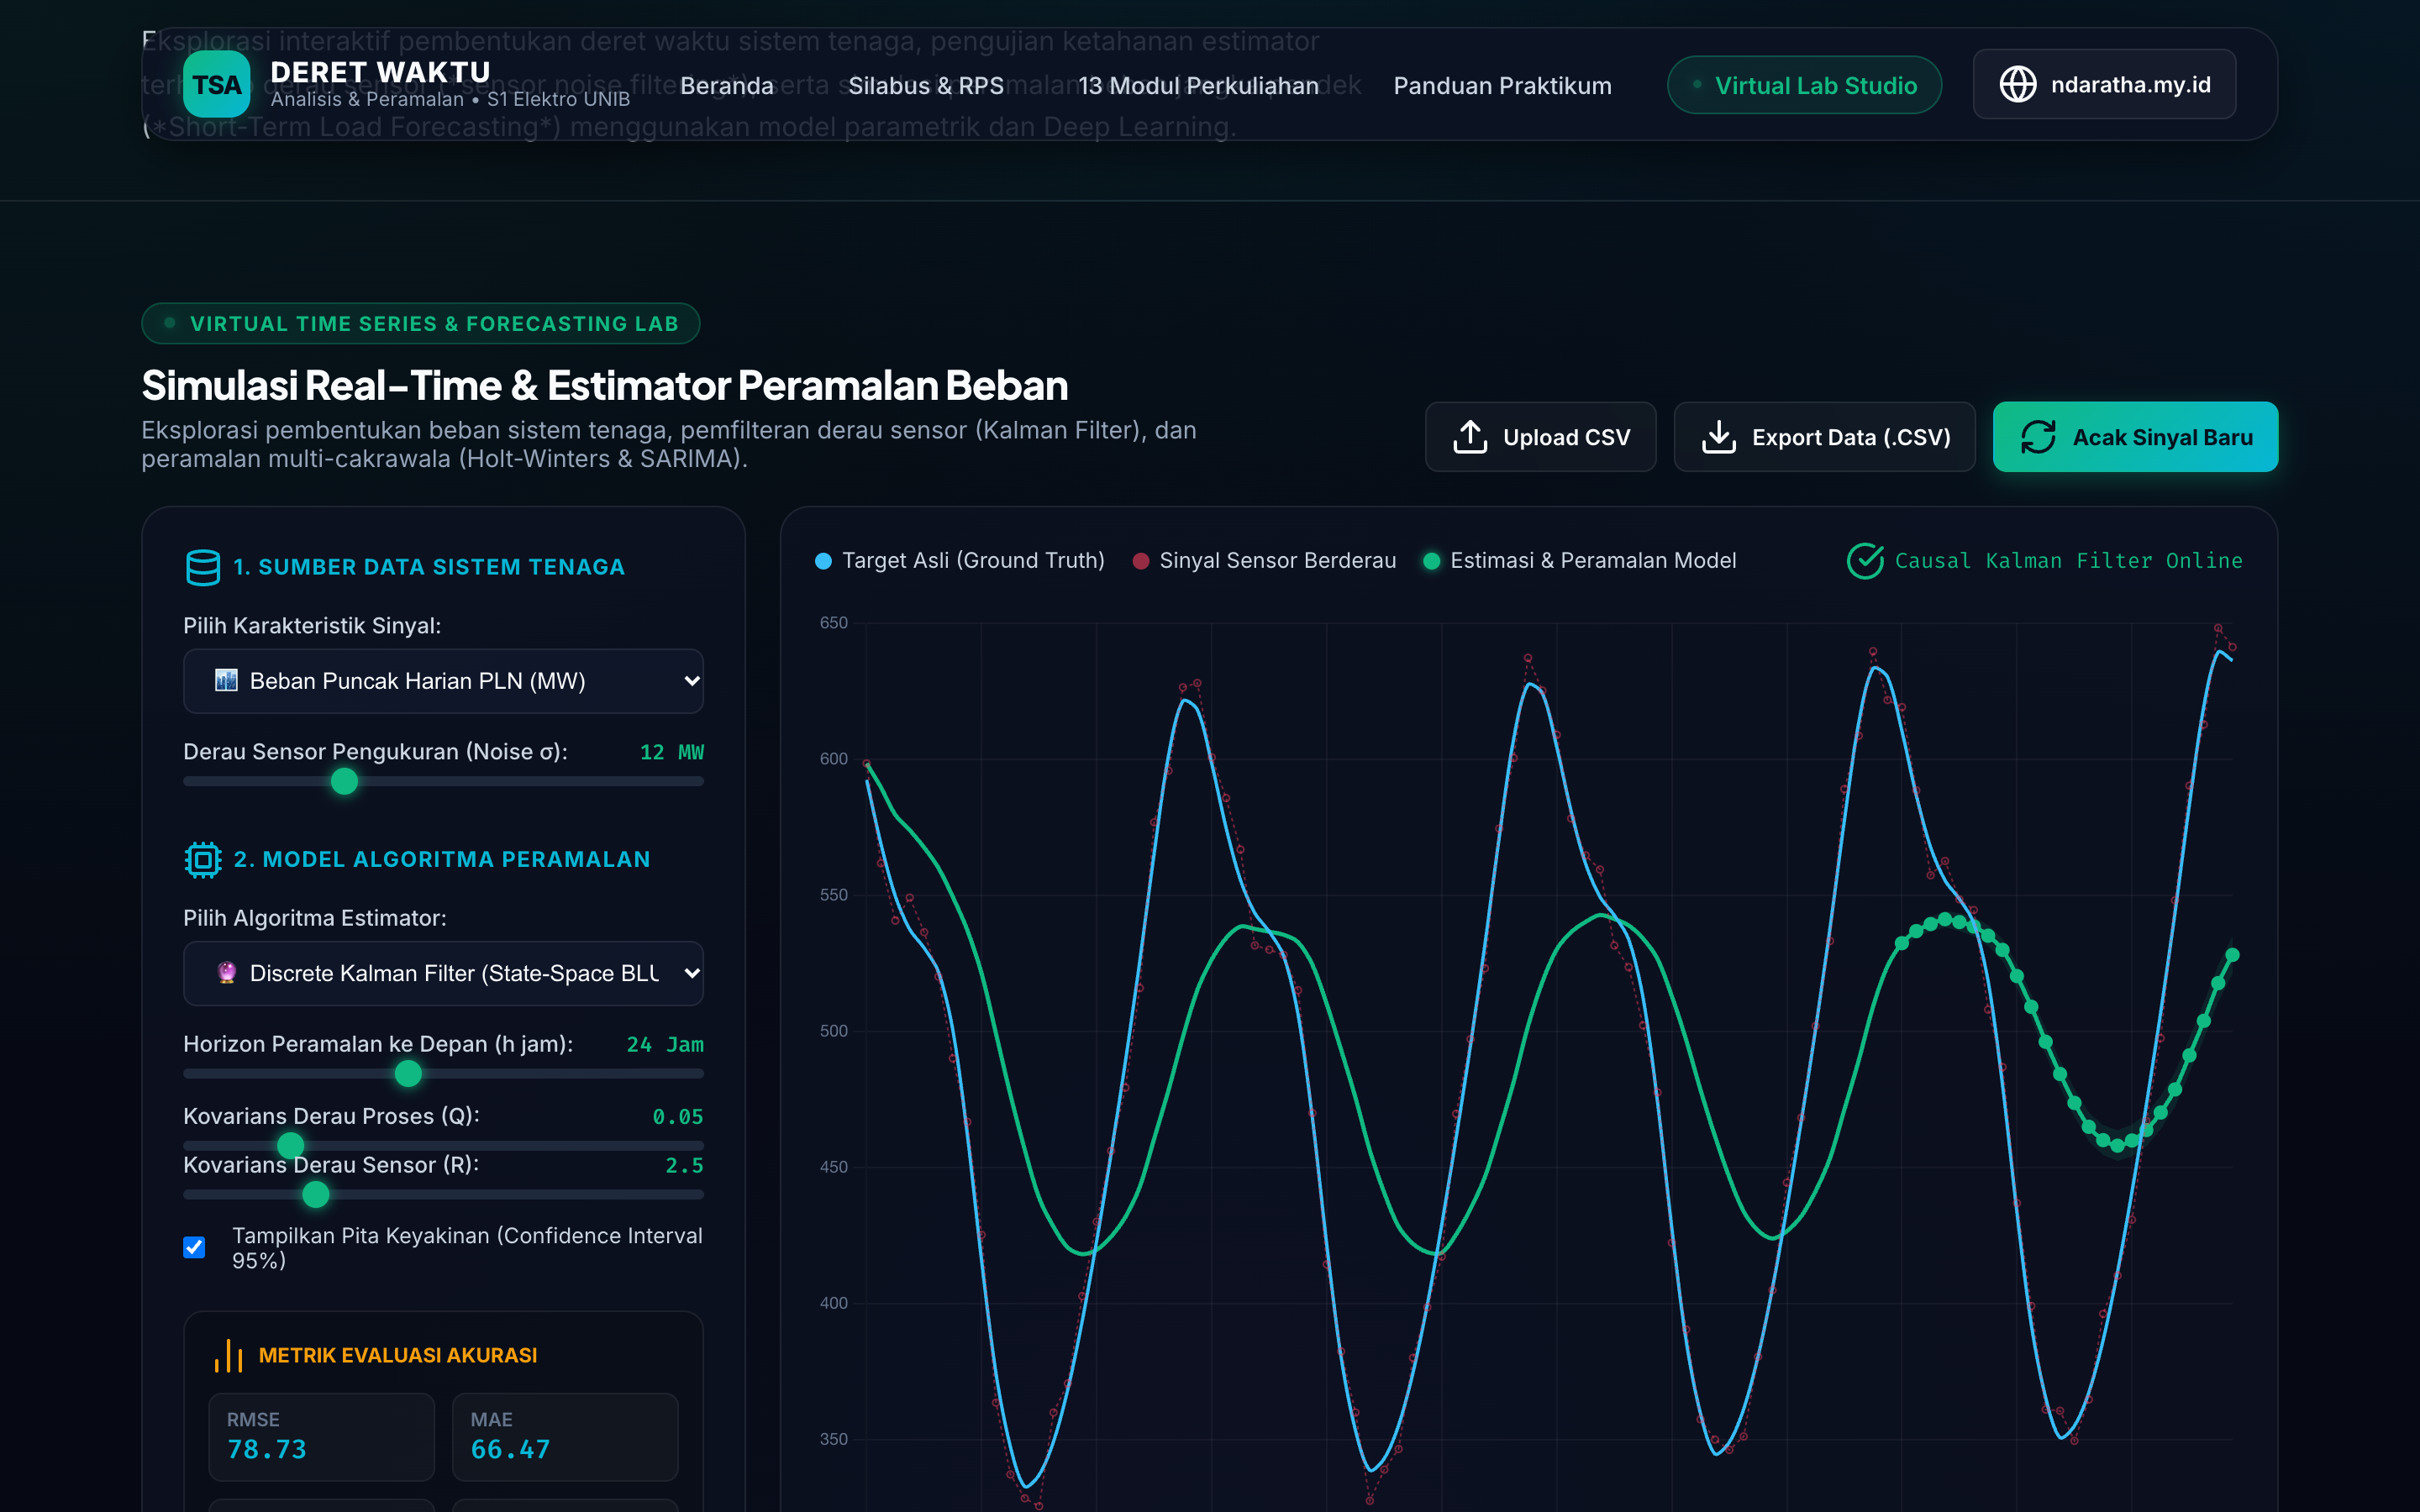
\includegraphics[width=0.92\textwidth]{screenshots/02_virtual_studio.png}}
    \caption{Virtual Forecasting Studio berbasis browser (100\% kausal) dengan 4 estimator, metrik RMSE/MAE/MAPE/$R^2$, dan tombol Upload CSV Mandiri.}
\end{figure}

\newpage
\begin{figure}[h!]
    \centering
    \fbox{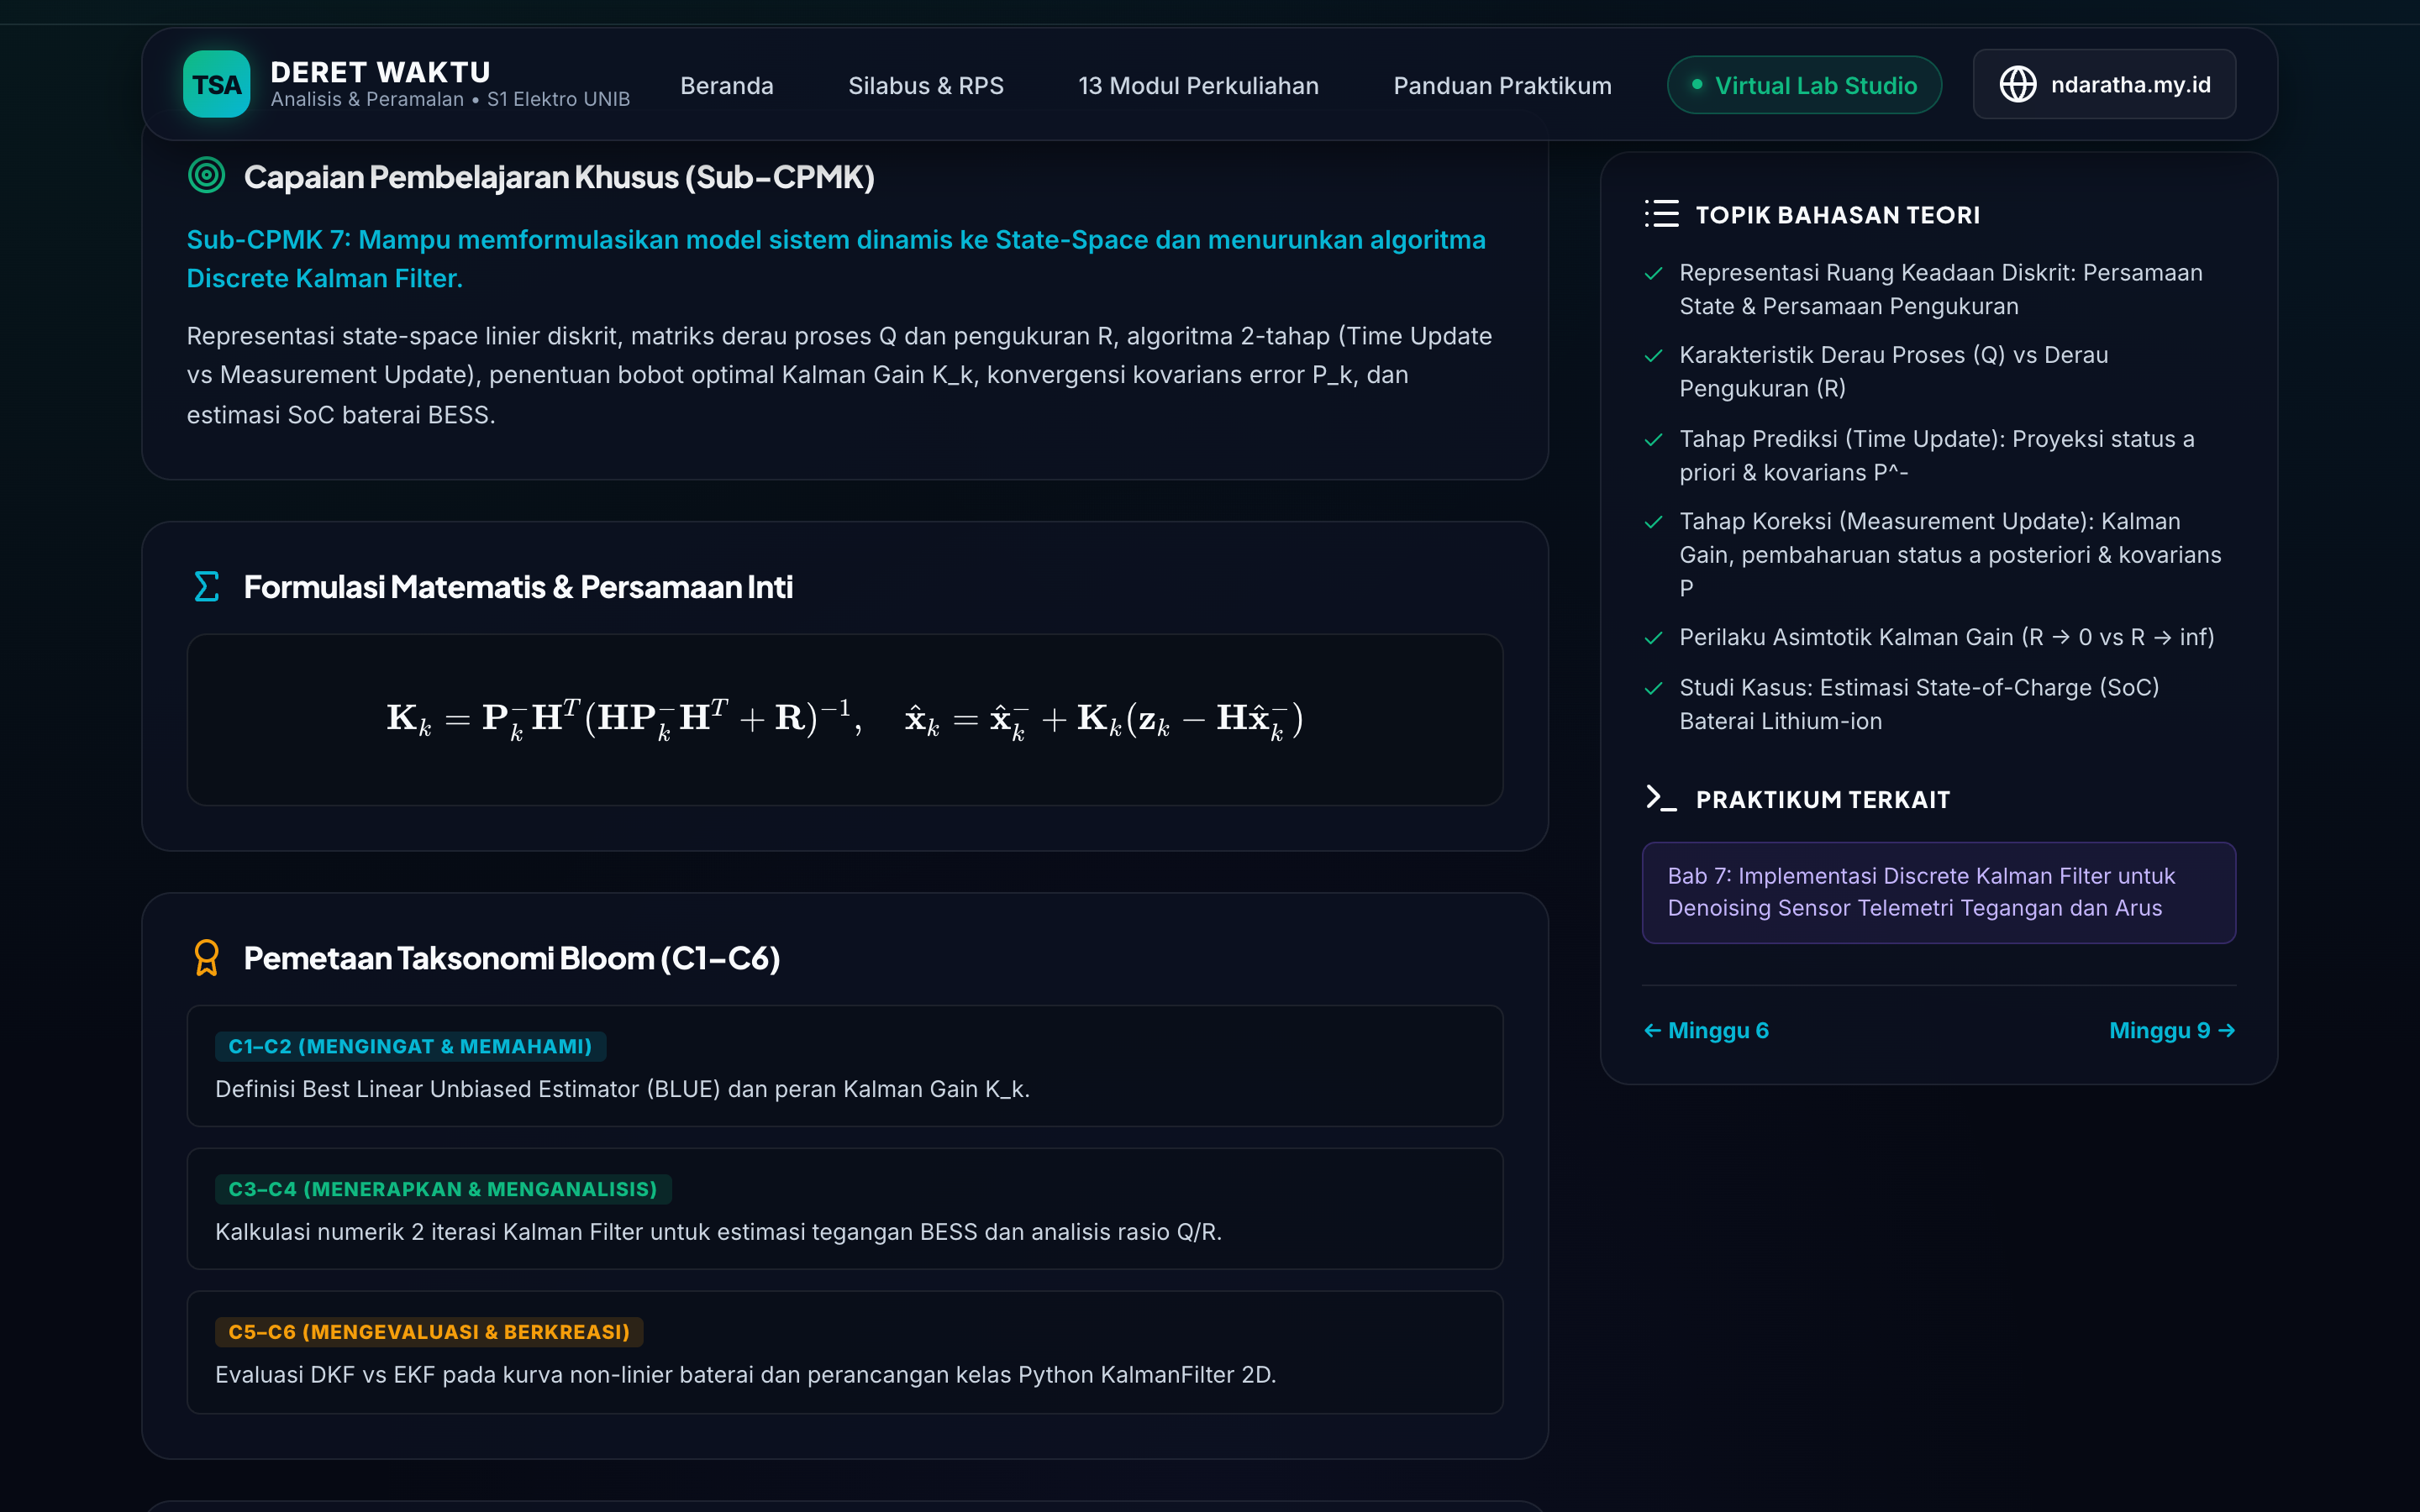
\includegraphics[width=0.92\textwidth]{screenshots/03_modul_kuis.png}}
    \caption{Halaman Modul Perkuliahan (Minggu 7: Discrete Kalman Filter) menampilkan formulasi KaTeX lokal, pemetaan Taksonomi Bloom C1--C6, kode Python, dan Kuis Self-Check Interaktif.}
\end{figure}

\begin{figure}[h!]
    \centering
    \fbox{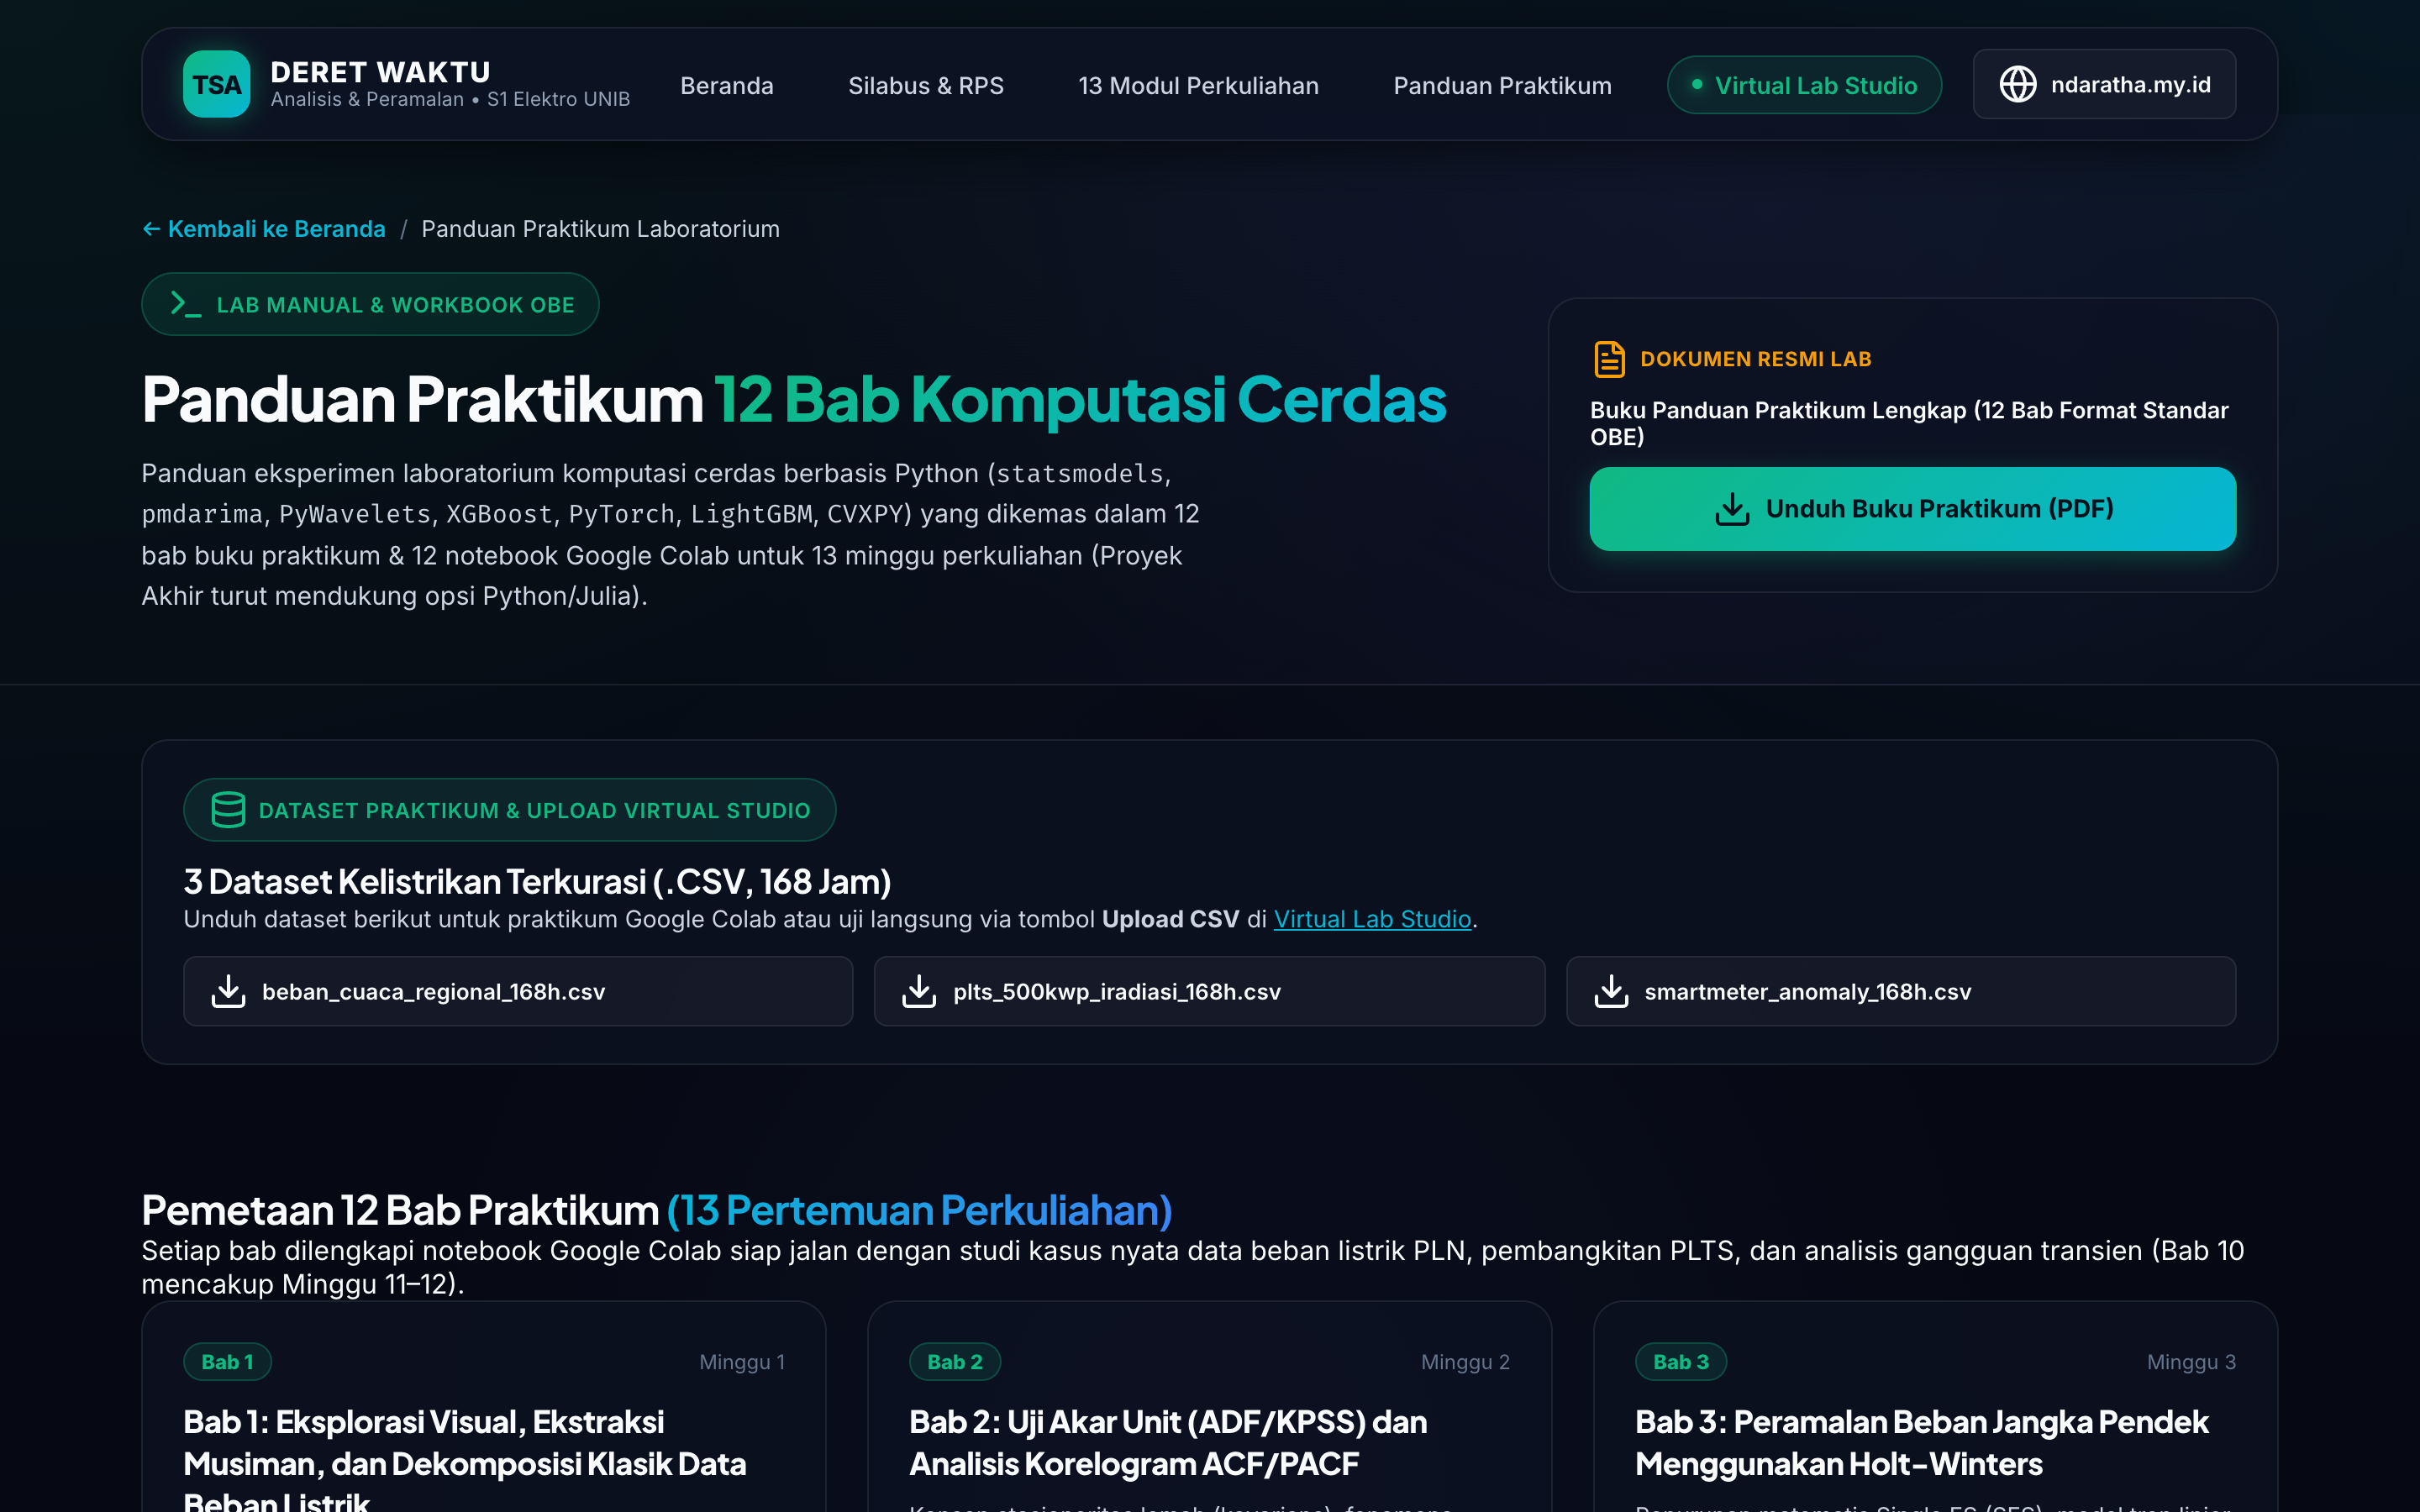
\includegraphics[width=0.92\textwidth]{screenshots/04_praktikum_colab.png}}
    \caption{Halaman Panduan Praktikum 12 Bab (13 Pertemuan) dilengkapi katalog 3 dataset CSV kelistrikan terkurasi dan tombol 1-klik Buka di Google Colab.}
\end{figure}

\end{document}
